%!TEX root = ../main.tex

\newenvironment{conditions}
  {\par\vspace{\abovedisplayskip}\noindent\begin{tabular}{>{$}l<{$} @{${}={}$} l}}
  {\end{tabular}\par\vspace{\belowdisplayskip}}


\tikzset{basic/.style={draw,fill=blue!50!green!20,
                       text badly centered,minimum width=3em}}
\tikzset{input/.style={basic,circle}}
\tikzset{weights/.style={basic,rectangle,minimum width=2em}}
\tikzset{functions/.style={basic,circle,fill=blue!50!green!20}}
\newcommand{\addsymbol}{\draw[thick] (0.5em,0.5em) -- (0,0.5em) -- 
                        (0,-0.5em) --  (-0.5em,-0.5em)
                        (0em,0.75em) -- (0em,-0.75em)
                        (0.75em,0em) -- (-0.75em,0em);}



\section{Εισαγωγή}

\subsection{Ορισμός}

Η έννοια της \textit{μηχανικής μάθησης} (\textit{machine learning}), ως κλάδος της επιστήμης των υπολογιστών, βρίσκεται στο επίκεντρο της σύγχρονης βιομηχανίας και έρευνας. Πρόκειται για μια μέθοδο ανάλυσης δεδομένων που αυτοματοποιεί την δημιουργία μοντέλων σε μηχανές και υπολογιστικά συστήματα, βοηθώντας στη σταδιακή βεκλτίωση της απόδοσής τους, χωρίς την παροχή συγκεκριμένων οδηγιών προκειμένου να το πετύχουν. Ουσιαστικά, αποτελεί μια εφαρμογή τεχνητής νοημοσύνης σε συστήματα, δίνοντάς τους τη δυνατότητα της μάθησης και της βελτίωσης της απόδοσής τους χωρίς να έχουν προγραμματισθεί για αυτό.

\medskip
Η μηχανική μάθηση, σαν όρος, αποδίδεται στον Αμερικανό \textit{Arthur Samuel}, που τον χρησιμοποίησε στη δημοσίευσή του το 1959 που αφορούσε τη δημιουργία έξυπνων αλγορίθμων μάθησης στο παιχνίδι της ντάμας \cite{Samuel1959}. Ένας πιο αυστηρός ορισμός των αλγορίθμων που ανήκουν στο πεδίο της μηχανικής μάθησης δόθηκε το 1997 από τον Αμερικανό επιστήμονα \textit{Tom M. Mitchell} και είναι ο εξής:

\medskip
\begin{displayquote}
Ενα πρόγραμμα υπολογιστή μαθαίνει από εμπειρία \textit{Ε} συναρτήσει κάποιων διεργασιών \textit{T} και απόδοσης \textit{P} αν η απόδοσή του \textit{P} σε όλες τις διεργασίες \textit{T} βελτιώνεται με την εμπειρία \textit{E}.
\end{displayquote}

\newpage
\subsection{Ιστορική Αναδρομή}

Προτού ωστόσο αποδοθεί ο όρος μηχανική μάθηση, είχαν ήδη δημιουργηθεί οι βάσεις για την ανάπτυξη του εν λόγω τομέα. Στατιστικές μέθοδοι είχαν ήδη αναπτυχθεί και βελτιστοποιηθεί. Το 1947 έχουμε την πρώτη αναφορά στον όρο \textit{νευρωνικά δίκτυα} από τους \textit{Warren McCulloch} και \textit{Walter Pitts} σε μια δημοσίευση αναφορικά με τους νευρώνες του εγκεφάλου και το πως λειτουργούν \cite{McCulloch1943}. Την ίδια περίοδο, ο \textit{Donald Hebb} στο βιβλίο του \textit{The Organization of Behaviour} που δημοσιεύτηκε το 1949 μοντελοποιεί τις αλληλεπιδράσεις μεταξύ των κυττάρων του εγκεφάλου και παράλληλα αναφέρει θεωρίες σχετικά με την ενεργοποίηση και την επικοινωνία των νευρώνων \cite{Hebb1967}. Σε αυτό το βιβλίο παρουσιάστηκε και για πρώτη φορά η έννοια του \textit{Hebbian learning}, που αποτελεί μια από τις βασικότερες θεωρίες στον χώρο της \textit{μη επιβλεπόμενης μάθησης} (στην οποία θα αναφερθούμε παρακάτω).

\medskip
Η δεκαετία του 1950 αποτέλεσε την απαρχή της ανάπτυξης αλγορίθμων μηχανικής μάθησης, με την εφαρμογή τους να πραγματοποιείται σε πολύ απλά προβλήματα. Ειδικότερα, το 1957 ο Αμερικανός ψυχολόγος και πρωτοπόρος στον χώρο της τεχνητής νοημοσύνης \textit{Frank Rosenblatt} συνδύασε τη θεωρία μοντελοποίησης των κυτταρικών αλληλεπιδράσεων του εγκεφάλου του \textit{D. Hebb} με τη θεωρία περί μηχανικής μάθησης του \textit{A. Samuel} και δημιούργησε τον αλγόριθμο \textit{Perceptron}, που αποτελεί έναν αλγόριθμο \textit{επιβλεπόμενης μάθησης} για δυαδική ταξινόμηση, με σκοπό τη χρήση του σε προβλήματα αναγνώρισης εικόνας (συγκεκριμένα αναγνώριση μοτίβων και σχημάτων).


\begin{figure}[h]
    \centering
    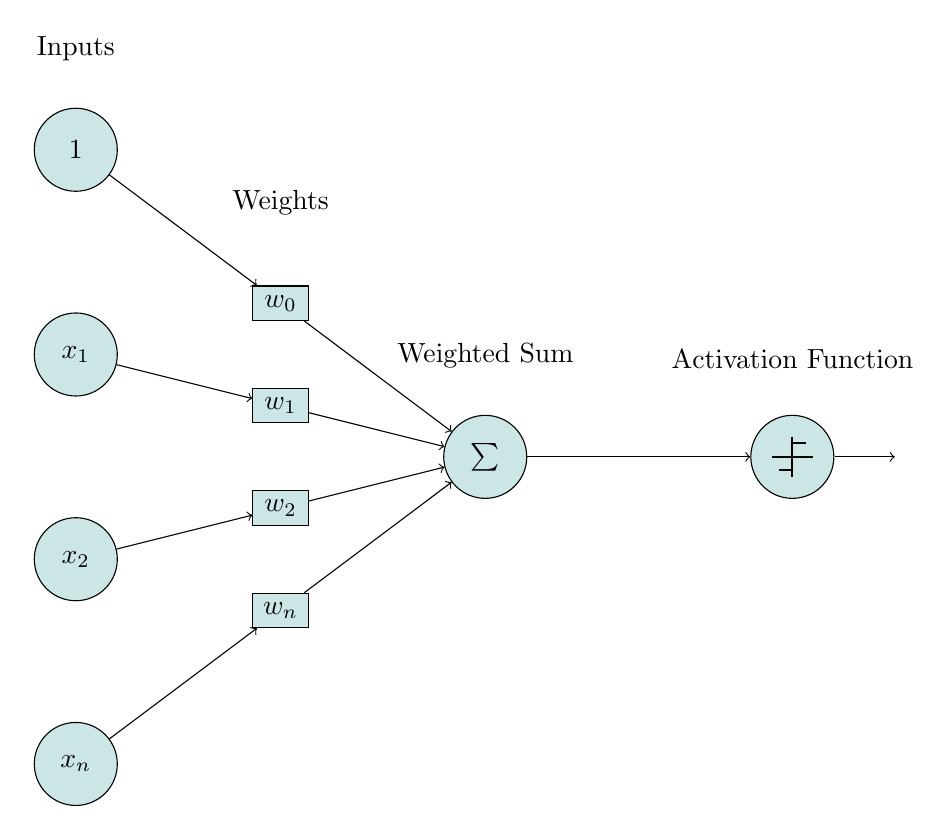
\begin{tikzpicture}[scale=1.3]
        \foreach \h [count=\hi ] in {$x_n$,$x_2$,$x_1$,$1$}{%
              \node[input] (f\hi) at (0,\hi*2cm-5 cm) {\h};
            }
        \node[functions] (sum) at (4,0) {$\sum$};
        \foreach \h [count=\hi ] in {$w_n$,$w_2$,$w_1$,$w_0$}{%
              \path (f\hi) -- node[weights] (w\hi) {\h} (sum);
              \draw[->] (f\hi) -- (w\hi);
              \draw[->] (w\hi) -- (sum);
            }        
        \node[functions] (step) at (7,0) {};
           \begin{scope}[xshift=7cm,scale=.75]
             \addsymbol
           \end{scope}
        \draw[->] (sum) -- (step);
        \draw[->] (step) -- ++(1,0);
        % Labels
        \node[above=1cm]  at (f4) {Inputs};
        \node[above=1cm] at (w4) {Weights};
        \node[above=1cm] at (sum) {Weighted Sum};
        \node[above=1cm] at (step) {Activation Function};
    \end{tikzpicture}
    \caption{Δομή του Perceptron}
    \label{fig: Δομή του Perceptron}
\end{figure}

\medskip
Η δεκαετία του 1960 είδε την εισαγωγή μπεϋζιανών μεθόδων στην μηχανική μάθηση καθώς και την εισαγωγή πολλαπλών επιπέδων στους ήδη υπάρχοντες αλγορίθμους μηχανικής μάθησης. Παράλληλα, το 1967 αναπτύχθηκε o αλγόριθμος \textit{Nearest Neighbor} \cite{Cover1967}. Ο αλγόριθμος χρησιμοποιήθηκε αρχικά σε προβλήματα χαρτογράφησης διαδρομών και αποτέλεσε την απαρχή της βασικής αναγνώρισης προτύπων.

\medskip
Ακολούθησε μια περίοδος στασιμότητας για την έρευνα και την ανάπτυξη της μηχανικής μάθησης, γεγονός που οφείλεται κυρίως στον σκεπτικισμό γύρω από τους περιορισμούς που είχαν όλες οι μέθοδοι, περιορισμοί άρρηκτα συνδεδεμένοι με τους περιορισμούς επεξεργαστικής δύναμης της εποχής. Μέσα σε αυτό το κλίμα αναπτύχθηκε το 1970 από τον Φινλανδό μαθηματικό \textit{Seppo Linnainmaa} η ιδέα του \textit{reverse automatic differentiation}, που αντιστοιχεί στην σύγχρονη έννοια του \textit{backpropagation} (αν και δεν ονομάστηκε έτσι πριν το 1986) \cite{Linnainmaa1976}. Ειδικότερα, η ιδεά περιγράφει την οπισθοδρομική διάδοση του σφάλματος, με το σφάλμα να υπολογίζεται στην έξοδο και να επανατροφοδοτείται σε επίπεδα του δικτύου για λόγους μάθησης.

\medskip
Η δεκαετία του 1980 είδε την εισαγωγή πολλών νέων και βασικών αλγορίθμων και θεωριών στον τομέα της μηχανικής μάθησης. Το 1982 ο Αμερικανός επιστήμονας \textit{John Hopfield} αναπτύσει τη θεωρία των \textit{associative neural networks}, που αποτελούν την πρώτη μορφή \textit{recurrent neural networks}, μιας αρχιτεκτονικής νευρωνικών δικτύων με μεγάλη διάδοση τις επόμενες δεκαετίες. 

\medskip
Ένας άλλος λόγος που η ανάπτυξη της μηχανικής μάθησης αντιμετώπισε μια στασιμότητα τις τελευταίες δεκαετίες ήταν η επικέντρωση της έρευνας σε γνωσιοκεντρικές (knowledge-based) προσεγγίσεις. Αυτό άλλαξε τη δεκαετία του 1990 όπου η έρευνα μετατοπίστηκε σε προσεγγίσεις με βάση τα δεδομένα (data-driven). Το 1995 δημοσιεύεται η εργασία της \textit{Tin Kam Ho} όπου παρουσιάζονται οι αλγόριθμοι κατηγοριοποίησης \textit{random forest} \cite{Ho}. Το 1995 γίνεται η σύγχρονη διατύπωση άλλης μιας σημαντικής θεωρίας, αυτής των \textit{support vector machines}, που αποτελούν μοντέλα επιβλεπόμενης μάθησης με χρήση σε προβλήματα κατηγοριοποίησης ή regression \cite{Cortes1995}. Παράλληλα, μια σημαντική τεχνική που χρησιμοποείται κατα κόρον μέχρι και σήμερα για την αναγνώριση ομιλίας αναπτύχθηκε το 1997 από τους \textit{Jürgen Schmidhuber} και \textit{Sepp Hochreiter}. Πρόκειτα για τα μοντέλα νευρωνικών δικτών \textit{Long Short-Term Memory}, που αποτελούν μια ειδική περίπτωση των προαναφερθέντων reccurent neural networks, με την ικανότητα να μαθαίνουν διεργασίες που απαιτούν μνήμη χιλλιάδων διακριτών βημάτων \cite{Hochreiter1997}.

\medskip
Κάπως έτσι, φτάνουμε στον 21\^ο αιώνα, και ειδικότερα μέτα το 2010, όπου η ραγδαία αύξηση της υπολογιστικής ισχύος επιτρέπει τη δημιουργία \textit{deep neural network} αρχιτεκτονικών. Πλεον, η μηχανική μάθηση είναι διαδεδομένη σε πολλαπλούς τομείς και βρίσκει χρήση σε πληθώρα εφαρμογών και υπηρεσιών λογισμικού, ενώ η έρευνα πάνω στο αντικείμενο έχει αυξηθεί κατα κόρον, με τις εταιρίες να επενδύουν σημαντικά ποσά προκειμένου να μείνουν μπροστά από τον ανταγωνισμό.


\begin{figure}[h]
  \centering
  \includegraphics[scale=0.5]{images/SVM.jpg}
  \caption{Support Vector Machines}
  \label{fig:Support Vector Machines}
\end{figure}


\section{Είδη μηχανικής μάθησης}

Η μηχανική μάθηση χωρίζεται σε πολλά και ξεχωριστά είδη, με τα συστήματα που την χρησιμοποιούν ως εργαλείο να χωρίζονται ανάλογα με:

\medskip
\begin{itemize}
    \item την προσέγγισή τους ως προς τη "μάθηση"
    \item τον τύπο δεδομένων που δέχονται στην είσοδο
    \item τον τύπο δεδομένων που δίνουν ως έξοδο
    \item τον τύπο προβλημάτων/διεργασιών που καλούνται να επιλύσουν κ.α.
\end{itemize}

\medskip
Διακρίνονται τρεις κύριες κατηγορίες μηχανικής μάθησης ως προς τον παράγοντα "μάθηση": \textit{επιβλεπόμενη μάθηση} (supervised learning), \textit{μη επιβλεπόμενη μάθηση}  (unsupervised learning) και \textit{ενισχυτική μάθηση} (re\-inforcement learning).

\subsection{Επιβλεπόμενη Μάθηση}

Η επιβλεπόμενη μάθηση περιγράφει μια κατηγορία προβλημάτων, που περιλαμβάνουν τη δημιουργια μοντέλων με σκοπό την \textit{χαρτογράφηση} δεδομένων εισόδου σε μια επιθυμητή έξοδο. Ένας πιο αυστηρός ορισμός δίνεται στο βιβλίο \textit{Pattern Recognition and Machine Learning}  \cite{Bishop2006} και είναι ο ακόλουθος:

\medskip
\begin{displayquote}
Applications in which the training data comprises examples of the input vectors along with their corresponding target vectors are known as supervised learning problems. 
\end{displayquote}

\medskip
Τα μοντέλα εκπαιδεύονται σε δεδομένα "εκπαίδευσης", που αποτελούνται από τα αντικείμενα εισόδου και τις επιθυμητές τιμές εξόδου τους, και χρησιμοποιούνται για να κάνουν προβλέψεις σε "τεστ" δεδομένα, όπου παρέχεται μόνο το κομμάτι της εισόδου και το αποτέλεσμα της πρόβλεψης συγκρίνεται με τις πραγματικές τιμές εξόδου προκειμένου να υπολογιστεί η ακρίβεια του μοντέλου.

\medskip
Υπάρχουν δύο βασικοί τύποι προβλημάτων επιβλεπόμενης μάθησης και διαφοροποιούνται με βάση το είδος της εξόδου που καλούνται να προβλέψουν. Συγκεκριμένα, ονομάζονται \textit{classification} τα προβλήματα που καλούνται να προβλέψουν μια κατηγορική έξοδο, ενώ ονομάζονται \textit{regression} όταν καλούνται να προβλέψουν μια αριθμητική τιμή.

\medskip
\begin{figure}[h]
  \centering
  \includegraphics[scale=0.3]{images/suplearn.png}
  \caption{Επιβλεπόμενη Μάθηση}
  \label{fig:suplearn}
\end{figure}

\subsection{Μη Επιβλεπόμενη Μάθηση}

Η μη επιβλεπόμενη μάθηση αναφέρεται σε προβλήματα που περιλαμβάνουν την ανάπτυξη μοντέλων για την περιγραφή ή την εξαγωγή σχέσεων από δεδομένα. Αποτελεί το αντίθετο της επιβλεπόμενης μάθησης, με την έννοια ότι δεν περιλαμβάνονται οι επιθυμητές τιμές στην εκπαίδευση του μοντέλου. Αντίθετα, τροφοδοτούμε το μοντέλο με μια πληθώρα δεδομένων και παρέχονται τα εργαλεία προκειμένου αυτό να κατανοήσει τις ιδιότητες των δεδομένων. Ύστερα, το μοντέλο μαθαίνει να ομαδοποιεί/οργανώνει τα δεδομένα με τέτοιον τρόπο ώστε κάποιος άνθρωπος να μπορεί να εξάγει συμπεράσματα για αυτά με βάση τη νέα οργάνωσή τους.

\medskip
Αποτελεί πολύ σημαντικό αντικείμενο στον τομέα της μηχανικής μάθησης, καθώς τα περισσότερα δεδομένα στον κόσμο είναι ανοργάνωτα και ασυσχέτιστα μεταξύ τους, επομένως η δυνατότητα υπολογιστικών συστημάτων να εξάγουν συμπεράσματα για αυτά αποτελεί πλεονέκτημα σε πολλές βιομηχανίες.

\medskip
Παρ' ότι υπάρχουν πολλές κατηγορίες μη επιβλεπόμενης μάθησης, οι κυριότερες είναι το \textit{clustering}, που περιλαμβάνει την εύρεση ομαδοποιήσεων σε ανοργάνωτα δεδομένα και το \textit{density estimation}, δηλαδή την εξαγωγή συμπερασμάτων σχετικά με την κατανομή των δεδομένων.

\medskip
\begin{figure}[h]
  \centering
  \includegraphics[scale=0.33]{images/unsuplearn.png}
  \caption{Μη Επιβλεπόμενη Μάθηση}
  \label{fig:unsuplearn}
\end{figure}

\subsection{Ενισχυτική Μάθηση}

Η ενισχυτική μάθηση περιγράφει μια κατηγορία προβλημάτων όπου ένας πράκτορας ενεργεί σε ένα περιβάλλον και πρέπει να \textit{μάθει} να λειτουργεί προκειμένου να μεγιστοποιήσει κάποιο κέρδος. Πιο συγκεκριμένα, η ενισχυτική μάθηση έχει τον ακόλουθο ορισμό:

\medskip
\begin{displayquote}
Reinforcement learning is learning what to do - how to map situations to actions - so as to maximize a numerical reward signal. The learner is not told which actions to take, but instead must discover which actions yield the most reward by trying them \cite{RichardS.Sutton2018}. 
\end{displayquote}

\medskip
Η διαδικασία μάθησης στη συγκεκριμένη μέθοδο παρομοιάζεται με τον τρόπο που οι άνθρωποι μαθαίνουν εμπειρικά από τα λάθη τους. Ο πράκτορας τοποθετείται σε ένα περιβάλλον και αρχικά πραγματοποιεί πολλά λάθη. Ωστόσο, εφόσον υπάρχει κάποιο σήμα προς τον πράκτορα που συσχετίζει τις σωστές συμπεριφορές με κάποια ανταμοιβή και τις λάθος με καποια ποινή, ενισχύεται η προτίμηση στις καλές συμπεριφορές. Ως αποτέλεσμα, με το πέρασμα του χρόνου ο αλγόριθμος μάθησης πραγματοποιεί λιγότερα λάθη απ' ότι προηγουμένως. Συνήθως υλοποιείται μέσω μοντέλων αποφάσεων Markov, που αποτελούν στοχαστικές διαδικασίες διακριτού χρόνου για τη μοντελοποίηση λήψης αποφάσεων.

\medskip
\begin{figure}[h]
  \centering
  \includegraphics[scale=0.78]{images/reinflearn.png}
  \caption{Ενισχυτική Μάθηση}
  \label{fig:reinflearn}
\end{figure}

\newpage
\section{Νευρωνικά Δίκτυα}

Τα νευρωνικά δίκτυα (\textit{Artificial Neural Networks}) βρίσκονται στο επίκεντρο της μηχανικής μάθησης και αποτελούν την πιο διαδεδομένη μορφή αλγορίθμων που υλοποιούν μοντέλα μάθησης. Πρόκειται για υπολογιστικά συστήματα που είναι σχεδιασμένα ώστε να "μιμούνται" τη λειτουργία των νευρικών δικτύων που υπάρχουν στους εγκεφάλους των ζωϊκών οργανισμών. Μαθαίνουν να υλοποιούν διεργασίες εξάγωντας χαρακτηριστικά από τα παραδείγματα που τους τροφοδοτούνται, δίχως να γνωρίζουν λεπτομέριες για τις διεργασίες και χωρίς να τους ορίζονται σαφείς κανόνες για τον τρόπο επίλυσης \cite{Chen2019}.

\medskip
Η απαρχή της θεωρίας των νευρωνικών δικτύων ήρθε, όπως αναφέρθηκε προηγουμένως, το 1947 από τους \textit{Warren McCulloch} και \textit{Walter Pitts}, που δημιούργησαν το πρώτο υπολογιστικό μοντέλο με βάση τα νευρωνικά δίκτυα. Το 1949 ο \textit{Donald Hebb} δημιουργεί ένα μοντέλο μάθησης (\textit{Hebbian Learning}) που βασίζεται στην ικανότητα των νευρώνων να τροποποιούν τη δομή και τη λειτουργία τους για να προσαρμοστούν σε περιβαλλοντικές αλλαγές (\textit{neural plasticity}), με τους \textit{W. Clark} και \textit{B. Farley} να υλοποιούν το παραπάνω μοντέλο μάθησης του Hebb σε υπολογιστικά συστήματα, γνωστά ως \textit{calculators} \cite{Farley1954}.

\subsection{Νευρώνες}

Τα νευρωνικά δίκτυα καθιστώνται από τεχνητούς νευρώνες, που αποτελούν το ανάλογο των βιολογικών νευρώνων. Ενας \textit{νευρώνας} αποτελεί ένα από τα βασικότερα στοιχεία του νευρικού συστήματος και πρόκειται για ένα κύτταρο που λαμβάνει, επεξεργάζεται και μεταδίδει πληροφορία μέσω ηλεκτρικών και χημικών σημάτων.

\medskip
\begin{figure}[h]
  \centering
  \includegraphics[scale=0.95]{images/neuron-structure.jpg}
  \caption{Βιολογική Δομή Νευρώνα}
  \label{fig:neuron-structure}
\end{figure}

\medskip
Σε δομικό επίπεδο, διακρίνονται τρια βασικά μέρη που αποτελούν έναν νευρώνα:

\begin{itemize}
    \item το κυτταρικό σώμα,
    \item τους δεδνδρίτες και
    \item τον άξονα.
\end{itemize}

\medskip
Το κυτταρικό σώμα αποτελεί το κεντρικό μέρος του νευρώνα, περιέχει τον πυρήνα του κυττάρου καθώς και άλλα οργανίδια που επιτρέπουν πρωτεϊνική σύνθεση (π.χ. endoplasmic reticulum) και παραγωγή ενέργειας (μιτοχόνδρια). Μέσω των δενδριτών και του άξονα, ένας νευρώνας επεκτείνει τις διεργασίες του σε άλλα κύτταρα. Οι δενδρίτες συνήθως διακλαδώνονται έντονα με σταδιακή μείωση στο πάχος τους έπειτα από κάθε διακλάδωση και περιέχουν το κύριο μέρος της πληροφορίας εισόδου του νευρώνα.Ο άξονας είναι πιο λεπτός και μπορεί να επεκταθεί εως και χιλίαδες φορές όσο η διάμετρος του κυτταρικού σώματος σε μήκος, ενώ μεταφέρει νευρικά σήματα μακριά από το σώμα και προς άλλα κύτταρα.

\medskip
Οσον αφορά τη λειτουργία τους, η πληροφορία εισέρχεται ως ηλεκτρική διέγερση μέσω των δενδριτών στο σώμα του νευρώνα, επεξεργάζεται και στη συνέχεια μεταδίδεται μέσω του άξονα (που λειτουργεί πρακτικά ως καλώδιο) και καταλήγει στα άκρα του, όπου και μεταδίδει την πληροφορία σε άλλα κύτταρα μέσω δομών που ονομάζονται \textit{συνάψεις}.

\subsection{Λειτουργία και Οργάνωση}

Στα ANNs, οι νευρώνες αποτελούν ένα είδος συνάρτησης που εκτελέι ένα weighted sum πάνω στις εισόδους τους και στη συνέχεια εφαρμόζουν έναν μη γραμμικό μετασχηματισμό στο αποτέλεσμα, το οποίο και μεταδίδουν στους νευρώνες με τους οποίους είναι συνδεδεμένοι. 

Αν θεωρήσουμε ως \(y\) την έξοδο ενός νευρώνα, η παραπάνω περιγραφή μοντελοποιείται μαθηματικά ως:
\begin{equation}
    y = f(\sum (x_1*w_1 + x_2 * w_2 + ... + x_n*w_n))
\end{equation}
where:

{
\centering
\begin{conditions}
   x_{n} & είσοδοι του νευρώνα \\
   w_{n} & βάρη του νευρώνα \\
   f(x) & συνάρτηση ενεργοποίησης του νευρώνα \\
\end{conditions}}

\medskip
Η συνάρτηση ενεργοποίησης είναι η συνάρτηση που περιγράφει την έξοδο του νευρώνα. Αποτελεί τον παράγοντα που εισάγει τη μη γραμμικότητα στη λειτουργία των νευρωνικών δικτύων και επομένως επιτρέπει την περιγραφή πολύπλοκων συστημάτων, διατηρώντας ωστόσο την επεξεργασία των εισόδων με απλό τρόπο. Οι συνηθέστερες συναρτήσεις ενεργοποίησης είναι οι βηματικές συναρτήσεις (\textit{step}), οι σιγμοειδής (\textit{sigmoid}) και οι συναρτήσεις γραμμικής ανόρθωσης (\textit{rectified linear units - ReLU }).

\begin{itemize}
    \item \textbf{Βηματικές συναρτήσεις}: Η έξοδος είναι δυαδική και παίρνει τιμή ανάλογα με το αν το weighted sum είναι πάνω ή κάτω από ένα ορισμένο κατώφλι $θ$.
    \begin{equation}
        y =
        \begin{cases}
        0 & if \sum(x_n*w_n) <  $θ$ \\
        1 & if \sum(x_n*w_n) >  $θ$ \\
        \end{cases}
    \end{equation}
    
    \item \textbf{Σιγμοειδείς συναρτήσεις}: Πρόκειται για φραγμένες,διαφορίσιμες και πραγματικές συναρτήσεις με χαρακτηριστική S-μορφή που χρησιμοποιούνται κυρίως για την υπολογιστική τους απλότητα. Ένα απλό παράδειγμα είναι η logistic function που έχει την ακόλουθη μορφή:
    \begin{equation}
        y = \frac{1}{1 + e^{-x}} = \frac{e^{x}}{e^{x} + 1}
    \end{equation}
    
    \item \textbf{Συναρτήσεις γραμμικής ανόρθωσης}: Αποτελεί πλέον την πιο διαδεδομένη συνάρτηση ενεργοποίησης για πολλούς τύπους νευρωνικών δικτύων καθώς αντιμετωπίζει πολλά προβλήματα παραγώγισης που εμφανίζουν οι σιγμοειδής (π.χ. vanishing gradients κ.α.). Ο μαθηματικός τους ορισμός είναι ο εξής:
    \begin{equation}
        y = \max(0,x)
    \end{equation}
\end{itemize}


\medskip
\begin{figure}[h]
  \centering
  \includegraphics[scale=0.4]{images/sneuron.png}
  \caption{Μαθηματική δομή τεχνητού νευρώνα}
  \label{fig:sneuron}
\end{figure}

\medskip
Οι νευρώνες συνήθως οργανόνονται σε πολλαπλά επίπεδα, με τους νευρώνες ενός επιπέδου να συνδέονται μόνο με τους νευρώνες του αμέσως προηγούμενου και του αμέσως επόμενου επιπέδου. Το πρώτο επίπεδο των νευρωνικών δικτύων, δηλαδή το επίπεδο των νευρώνων που δέχεται την είσοδο, ονομάζεται \textit{επίπεδο εισόδου}, ενώ το επίπεδο που παρέχει τις εξόδους του νευρωνικού δικτύου ονομάζεται \textit{επίπεδο εξόδου}. Ενδιάμεσα μπορεί να μεσολαβούν κανένα, ένα ή και περισσότερα επίπεδα αναλόγως με την πολυπλοκότητα του δικτύου. Παράλληλα, ο τρόπος σύνδεσης των νευρώνων μεταξύ διαφορετικών επιπέδων μπορεί να διαφέρει. Μπορεί να είναι \textit{πλήρως διασυνδεδεμένα}, δηλαδή κάθε νευρώνας ενός επιπέδου να συνδέεται με όλους τους νευρώνες του επόμενου επιπέδου είτε να υπάρχουν για π.χ. επίπεδα \textit{pooling}, οπου μια ομάδα νευρώνων από ένα επίπεδο να συνδέεται σε έναν νευρώνα του επόμενου επιπέδου, μειώνοντας τον αριθμό των νευρώνων σε αυτο το επίπεδο.

\medskip
Ένας άλλος παράγοντας για την ορθή λειτουργία των νευρωνικών δικτύων είναι οι λεγόμενες \textit{υπερπαράμετροι}. Οι υπερπαράμετροι αποτελούν παραμέτρους που ορίζονται πριν την διαδικασία μάθησης των μοντέλων. Αν και δεν επηρεάζουν την απόδοση του μοντέλου, έχουν επίδραση πάνω στην ταχύτητα σύγκλισης και στην ποιότητα της μάθησης. Μερικά παραδείγματα υπερπαραμέτρων είναι ο \textit{ρυθμός μάθησης}, ο αριθμός \textit{κρυφών} επιπέδων και το \textit{batch size}.

\subsection{Αρχιτεκτονικές νευρωνικών δικτύων}

Η εξέλιξη της τεχνολογίας έχει επιτρέψει την άνοδο πολλών αρχιτεκτονικών νευρωνικών δικτύων, οι οποίες με τη σειρά τους έχουν πετύχει state-of-the-art αποτελέσματα σε πολλαπλούς τομείς.

Η πρώτη και απλούστερη δομή νευρωνικών δικτύων είναι η \textit{feedfor\-ward} αρχιτεκτονική. Στη συγκεκριμένη δομή, η πληροφορία κινείται μονάχα προς μια κατεύθυνση, από το επίπεδο εισόδου προς το επίπεδο εξόδου μέσω των κρυφών επιπέδων (αν υπάρχουν).

\medskip
\begin{figure}[h]
  \centering
  \includegraphics[scale=0.7]{images/Feedforward.jpg}
  \caption{Feedforward αρχιτεκτονική}
  \label{fig:feedforward}
\end{figure}

Αυτή η μονοδιάστατη ροή πληροφορίας άλλαξε με την είσοδο στον χώρο των \textit{recurrent neural networks}. Αποτελούν μια δομή νευρωνικών δικτύων όπου εκτός από την εμπρόσθια ροή της πληροφορίας, δίνεται η δυνατότητα στους νευρώνες να χρησιμοποιήσουν την εσωτερική τους κατάσταση για να αξιολογήσουν δεδομένα εισόδου, με αποτέλεσμα την ροή πληροφορίας και προς τα πίσω. Τα recurrent neural networks αποτελούν πλέον την πιο διαδεδομένη μορφή νευρωνικών δικτύων για χρήση σε προβλήματα επεξεργασίας φυσικής γλώσσας, επεξεργασίας ομιλίας καθώς και αναγνώρισης γραφικού χαρακτήρα.

\medskip
\begin{figure}[h]
  \centering
  \includegraphics[scale=0.65]{images/recurrent.png}
  \caption{Recurrent αρχιτεκτονική}
  \label{fig:recurrent}
\end{figure}

\medskip
Μια ακόμη διαδεδομένη μορφή νευρωνικών δικτύων, που χρησιμοποιείται κατα κόρον σε προβλήματα επεξεργασίας εικόνων, είναι η αρχιτεκτονική \textit{συνελικτικών} νευρωνικών δικτύων (\textit{convolutional} neural networks). Ως συνελικτικά νευρωνικά δίκτυα θεωρούνται τα νευρωνικά δίκτυα που συμπεριλαμβάνουν επίπεδα όπου πραγματοποιείται συνέλιξη. Πρακτικά, απο μαθηματική άποψη σε ένα συνελικτικό επίπεδο πραγματοποιείται ένα εσωτερικό γινόμενο μιας περιοχής των εξόδων των νευρώνων του προηγούμενου επιπέδου με κάποια φίλτρα (που ορίζονται πριν την εκπαίδευση των μοντέλων), ακολουθεί ένα στάδιο \textit{pooling} οπου μειώνεται η διαστασιμότητα του μοντέλου και τα αποτελέσματα τροφοδοτούνται συνήθως σε πλήρως διασυνδεδεμένα επίπεδα.

\medskip
\begin{figure}[h]
  \centering
  \includegraphics[scale=1.2]{images/cnn.png}
  \caption{Convolutional αρχιτεκτονική}
  \label{fig:cnn}
\end{figure}

\medskip
Τέλος, αξίζει να αναφερθεί μια ακόμη αρχιτεκτονική που αναπτύχθηκε το 2014 από τον Ian Goodfellow και την ομάδα του \cite{Goodfellow2014}. Πρόκειται για τα \textit{General Adversarial Networks} (GANs) , τα οποία δοσμένου ενός σετ δεδομένων εκπαίδευσης μαθαίνουν να δημιουργούν νέα δεδομένα με τα ίδια στατιστικά χαρακτηριστικά με τα δεδομένα εκπαίδευσης. Όσον αφορά τη λειτουργία τους, δύο νευρωνικά δίκτυα "ανταγωνίζονται" το ένα το άλλο σε ένα "παιχνίδι", με το ένα δίκτυο (\textit{generative}) να παράγει υποψήφια νέα δεδομένα και το άλλο (\textit{discriminative}) να τα αξιολογεί. Τα GANs έχουν εξαιρετικά αποτελέσματα στην παραγωγή ρεαλιστικών φωτογραφιών, στο βαθμό που ένας άνθρωπος δεν μπορεί να ξεχωρίσει αν η φωτογραφία είναι πραγματική ή κατασκευασμένη. 

\medskip
\begin{figure}[h]
  \centering
  \includegraphics[scale=0.4]{images/gan.png}
  \caption{General Adversarial Network αρχιτεκτονική}
  \label{fig:gan}
\end{figure}

